\documentclass[conference]{IEEEtran}
\usepackage{cite}
\usepackage{amsmath,amssymb,amsfonts}
\usepackage{algorithmic}
\usepackage{graphicx}
\usepackage{textcomp}
\usepackage{xcolor}
\usepackage{hyperref}
\usepackage{booktabs}
\usepackage{multirow}
\usepackage{tikz}
\usetikzlibrary{shapes.geometric, arrows, positioning}

\def\BibTeX{{\rm B\kern-.05em{\sc i\kern-.025em b}\kern-.08em
    T\kern-.1667em\lower.7ex\hbox{E}\kern-.125emX}}

\begin{document}

\title{MuscleWalker: Bio-Inspired Musculoskeletal Locomotion Control Using Deep Reinforcement Learning and Model Predictive Control}

\author{
\IEEEauthorblockN{Keval Shah, Zhixian Xie, Gourav Khanduri, Maharshi Shukla, Sanskar Patil}
\IEEEauthorblockA{\textit{School of Computing and Augmented Intelligence}\\
\textit{Arizona State University}\\
Tempe, AZ, USA}
}

\maketitle

\begin{abstract}
This paper presents MuscleWalker, a bio-inspired robotics project that explores the control of bipedal locomotion using compliant muscle-tendon actuators. Unlike traditional robots driven by stiff torque motors, MuscleWalker simulates a musculoskeletal system where forces are generated by contracting muscles that pull on tendons, mimicking the biomechanics of humans and animals. We implement and compare two primary control strategies: Deep Reinforcement Learning using Proximal Policy Optimization (PPO) for robust walking, jogging, and jumping gaits, and Model Predictive Path Integral (MPPI) control for dynamic balance and short-horizon planning. Our simulation environment is built on MuJoCo, enabling high-fidelity physics simulation of the muscle-tendon dynamics. Results demonstrate that distinct gaits emerge purely from reward function shaping, and the compliant actuation provides natural robustness to disturbances. The project successfully achieves forward locomotion with speeds up to 1.0 m/s for walking and demonstrates the emergence of rhythmic jumping behaviors through properly designed reward structures.
\end{abstract}

\begin{IEEEkeywords}
Bio-inspired robotics, musculoskeletal locomotion, reinforcement learning, model predictive control, MuJoCo simulation
\end{IEEEkeywords}

\section{Introduction}

Bipedal locomotion represents one of the most challenging problems in robotics, requiring precise coordination of multiple degrees of freedom while maintaining dynamic balance. Traditional approaches to robot locomotion rely on stiff, high-gain actuators that directly control joint torques or positions. While this approach has achieved significant success in controlled environments, it fundamentally differs from biological locomotion systems, which utilize compliant muscles and tendons to generate movement.

Biological locomotion systems offer several advantages over traditional rigid actuators. The inherent compliance of muscles and tendons provides natural shock absorption, reducing the impact forces during ground contact. The series elasticity in the muscle-tendon unit stores and releases energy during cyclic motions, improving energy efficiency. Furthermore, the passive dynamics of compliant systems can simplify control requirements by automatically responding to perturbations without explicit feedback.

The MuscleWalker project addresses the challenge of controlling a simulated bipedal robot actuated by Hill-type muscle models connected to tendons with series elasticity. Unlike conventional motor-driven robots, this system requires the controller to coordinate antagonist muscle pairs that work together to generate net joint torques. The control problem becomes more complex because muscle forces depend on activation dynamics, muscle length, and contraction velocity.

We investigate two complementary control approaches for this challenging actuation system. The first approach uses deep reinforcement learning, specifically the Proximal Policy Optimization (PPO) algorithm, to learn control policies directly from experience. This model-free approach enables the discovery of effective gait patterns without requiring an accurate model of the complex muscle-tendon dynamics. The second approach employs Model Predictive Path Integral (MPPI) control, a sampling-based model predictive control method that uses the simulation model to predict future states and optimize control sequences.

The main contributions of this work include: (1) the design and implementation of a biologically-inspired bipedal robot model with Hill-type muscle actuators in MuJoCo; (2) custom Gymnasium environments for training reinforcement learning agents on walking, jogging, and jumping tasks; (3) a comparative analysis of PPO-based learning and MPPI-based planning for muscle-actuated systems; and (4) demonstration of emergent gait behaviors arising from carefully designed reward functions.

The remainder of this paper is organized as follows. Section II reviews related work in bio-inspired locomotion and control methods. Section III describes the musculoskeletal walker model and its components. Section IV presents the control methods used in this project. Section V details the experimental setup and reward function design. Section VI presents results and analysis. Section VII discusses findings and limitations. Section VIII concludes the paper.

\section{Related Work}

\subsection{Bio-Inspired Locomotion}

Bio-inspired locomotion has been a growing field in robotics research, drawing inspiration from biological systems to improve robot performance. Early work by Raibert demonstrated fundamental principles of dynamic legged locomotion using simplified models. More recently, researchers have explored soft robotic actuators and cable-driven systems that more closely mimic biological muscle architecture.

The use of series elastic actuators (SEAs) in legged robots has shown promise for improving energy efficiency and robustness. Pratt and colleagues introduced the concept of SEAs and demonstrated their benefits for walking robots. Building on this work, various researchers have developed actuators with tunable stiffness that can adapt to different locomotion requirements.

Hill-type muscle models, originally developed to describe biological muscle behavior, have been increasingly adopted in robotics simulations. These models capture the essential force-length and force-velocity relationships of biological muscles, enabling more realistic simulation of musculoskeletal systems. The OpenSim project has been particularly influential in providing tools for musculoskeletal modeling and simulation.

\subsection{Reinforcement Learning for Locomotion}

Deep reinforcement learning has emerged as a powerful approach for learning locomotion controllers. Early work by Schulman et al. on Trust Region Policy Optimization (TRPO) and subsequently Proximal Policy Optimization (PPO) provided stable policy gradient methods suitable for continuous control tasks. These algorithms have been successfully applied to a wide range of simulated locomotion problems.

The DeepMind Control Suite and OpenAI Gym have provided standardized benchmarks for evaluating locomotion learning algorithms. Work by Heess et al. demonstrated that rich motor behaviors could emerge from simple reward functions when trained with sufficient computational resources. More recent work has explored curriculum learning and hierarchical policies to tackle more complex locomotion tasks.

Transfer from simulation to real robots remains a significant challenge. Domain randomization approaches, introduced by Tobin et al., have shown promise for improving sim-to-real transfer. However, the complexity of muscle-tendon dynamics presents additional challenges for simulation fidelity that require careful consideration.

\subsection{Model Predictive Control}

Model Predictive Control (MPC) provides an alternative approach to locomotion control that explicitly uses a model of the system dynamics. Traditional MPC methods solve optimization problems at each timestep to determine optimal control actions. While effective, these methods can be computationally expensive and may struggle with non-convex optimization landscapes.

Sampling-based MPC methods, such as Model Predictive Path Integral (MPPI) control introduced by Williams et al., avoid explicit optimization by sampling many control trajectories and weighting them based on their costs. This approach has proven particularly effective for systems with complex dynamics and non-smooth cost functions. MPPI has been successfully applied to autonomous driving and quadrotor control, and more recently to legged locomotion.

The combination of learning and model-based control has also gained attention. Some approaches use learned models within MPC frameworks, while others combine learned policies with model-based refinement. Our work contributes to this literature by comparing pure learning and pure model-based approaches for muscle-actuated systems.

\section{System Description}

\subsection{Musculoskeletal Walker Model}

The MuscleWalker robot is modeled as a planar bipedal system consisting of a torso and two legs, each with a thigh, shank, and foot segment. The model is implemented in MuJoCo XML format, enabling efficient physics simulation with accurate contact dynamics.

The torso serves as the central body of the robot and contains three degrees of freedom relative to the world: horizontal translation (rootx), vertical translation (rootz), and pitch rotation (rooty). These free joints allow the robot to move through the environment without kinematic constraints. The torso is heavily damped to prevent excessive oscillations during locomotion.

Each leg consists of three joints: a hip joint connecting the thigh to the torso, a knee joint connecting the shank to the thigh, and an ankle joint connecting the foot to the shank. The hip joints allow rotation in the range of -45 to 135 degrees, enabling both hip extension for push-off and hip flexion for swing phase. The knee joints have a range of -150 to 0 degrees, consistent with the anatomically correct constraint that knees extend rather than hyperextend. The ankle joints allow ±45 degrees of rotation for plantar flexion and dorsiflexion.

\subsection{Muscle-Tendon Actuation}

Unlike conventional torque-controlled robots, MuscleWalker uses muscle actuators connected to tendons that span joints. Each joint is controlled by an antagonist pair of muscles: a flexor and an extensor. This arrangement mimics biological systems where opposing muscle groups work together to control joint motion.

The tendons in our model are implemented as spatial elements connecting attachment sites on adjacent body segments. Each tendon has specific spring parameters that define its passive elasticity. The flexor tendons are modeled as active tendons with zero passive stiffness, allowing muscles to pull through them. The extensor tendons have high stiffness values, providing passive resistance that works antagonistically with the active flexors.

The muscle actuators follow a simplified Hill-type model where the muscle force depends on the activation level and the tendon length. The control input to each muscle is an activation level between 0 and 1, where 0 represents no activation and 1 represents full activation. The muscle generates force proportional to its activation and the maximum force capacity defined in the model.

For the knee joints, the extensor tendons have a stiffness of 10,000 N/m to support the full body weight during stance. The hip extensor tendons have a stiffness of 5,000 N/m, while the ankle extensor tendons have the highest stiffness at 20,000 N/m to provide stable ground contact. These values were tuned empirically to achieve stable locomotion.

\subsection{Simulation Environment}

The simulation is implemented using MuJoCo, a physics engine designed for fast and accurate simulation of articulated rigid body systems with contacts. MuJoCo provides efficient computation of forward and inverse dynamics, contact detection and resolution, and tendon and muscle simulation.

The simulation runs at a timestep of 2.5 milliseconds, providing sufficient temporal resolution to capture the dynamics of muscle contractions and ground contacts. A frame skip of 10 is used during training, meaning the control policy operates at 40 Hz while the physics simulation runs at 400 Hz.

The ground is modeled as an infinite plane with friction coefficients of 0.7 for sliding, 0.1 for torsional, and 0.1 for rolling friction. These values provide realistic ground contact behavior while allowing smooth transitions between stance and swing phases.

\section{Control Methods}

\subsection{Proximal Policy Optimization}

We use Proximal Policy Optimization (PPO), a policy gradient method for deep reinforcement learning, to learn locomotion policies. PPO has become one of the most widely used algorithms for continuous control tasks due to its stability and sample efficiency.

The policy is represented as a multi-layer perceptron (MLP) network that maps observations to action distributions. The observation space includes the robot's generalized positions (excluding the horizontal position for translation invariance), generalized velocities, and muscle activation states when applicable. The observation dimension is 17 for models without activation dynamics and increases when internal muscle states are included.

The action space consists of six continuous values corresponding to the activation levels of the six muscles (right hip flexor, right knee flexor, right ankle flexor, left hip flexor, left knee flexor, left ankle flexor). The network outputs actions in the range [-1, 1], which are then scaled to [0, 1] for muscle activations.

Training uses the Stable Baselines3 implementation of PPO with the following hyperparameters: learning rate of 3e-4, batch size of 64, horizon of 2048 steps, discount factor of 0.99, and entropy coefficient of 0.01. The entropy bonus encourages exploration during early training.

The policy is trained using episodes with a maximum length of 1000 steps. Episodes can terminate early if the robot falls (defined as the height dropping below a threshold or the pitch angle exceeding safe limits). Early termination provides a strong learning signal to avoid falling behaviors.

\subsection{Model Predictive Path Integral Control}

As an alternative to learning-based control, we implement Model Predictive Path Integral (MPPI) control combined with a GPU-accelerated control strategy. MPPI is a sampling-based optimization method that evaluates many candidate control sequences and weights them based on their expected costs.

At each control timestep, MPPI generates a batch of control sequences by adding Gaussian noise to the current nominal control sequence. Each control sequence is rolled out using the simulation model to predict the resulting state trajectory. A cost function evaluates each trajectory, assigning lower costs to trajectories that achieve the desired behavior.

The control update is computed as a weighted average of the noise samples, where the weights are computed using softmax over the negative costs. Specifically, for trajectory $i$ with cost $c_i$, the weight is:
\begin{equation}
w_i = \frac{\exp(-c_i / \lambda)}{\sum_j \exp(-c_j / \lambda)}
\end{equation}
where $\lambda$ is a temperature parameter controlling the sharpness of the weighting.

Our implementation uses a planning horizon of 40 steps, 512 sample trajectories, temperature parameter of 0.01, and noise standard deviation of 1.0. The frame skip of 10 means the planning horizon corresponds to 1.0 seconds of simulated time.

The MPPI controller in this project is implemented using MuJoCo's batch rollout functionality, which efficiently simulates multiple trajectories in parallel using 32 threads. This parallelization is essential for real-time control, as evaluating 512 trajectories sequentially would be computationally prohibitive.

\subsection{Reward and Cost Function Design}

The reward function design is critical for both learning and model-based control approaches. For the walking task, we design a multiplicative reward structure that encourages forward progress while maintaining balance:

\begin{equation}
R_{\text{walk}} = R_{\text{standing}} \cdot R_{\text{move}}
\end{equation}

The standing reward combines multiple components:
\begin{equation}
R_{\text{standing}} = \frac{2 \cdot f_{\text{height}} + f_{\text{upright}} + f_{\text{knee}} + f_{\text{hip}}}{5}
\end{equation}

where $f_{\text{height}}$ penalizes deviation from the nominal height, $f_{\text{upright}}$ rewards vertical torso orientation, and $f_{\text{knee}}$ and $f_{\text{hip}}$ reward natural joint postures.

The movement reward is based on forward velocity:
\begin{equation}
R_{\text{move}} = \text{clip}\left(\frac{v_x}{v_{\text{target}}}, 0, 1\right)
\end{equation}

This multiplicative structure ensures that the robot must maintain balance (high $R_{\text{standing}}$) while also making forward progress (high $R_{\text{move}}$). A robot that falls or moves backward receives very low reward.

For the jumping task, we design a more complex reward that includes components for forward progress, height maintenance, flight phase rewards, takeoff bonuses, leg synchronization, action symmetry, and energy efficiency. The jumping reward encourages rhythmic hopping behavior where both feet leave and contact the ground simultaneously.

\section{Experimental Setup}

\subsection{Training Configuration}

All reinforcement learning experiments were conducted using PPO as implemented in Stable Baselines3. The training was performed on a workstation with multi-core CPU support. TensorBoard logging was used to monitor training progress and visualize learning curves.

For the walking task, the agent was trained for 100,000 timesteps as the default, with options to extend to 1,000,000 timesteps for improved performance. The environment resets when the robot falls (height below -0.5 or pitch exceeding 1.2 radians) or when the episode length exceeds 1000 steps.

For the jogging and jumping tasks, similar training configurations were used with task-specific reward functions. The jumping task used a frame skip of 40 (operating at 10 Hz) to allow sufficient time for the jumping dynamics to develop within the planning horizon.

\subsection{Evaluation Metrics}

We evaluate the learned and designed controllers using several metrics:

\textbf{Forward Speed:} The average forward velocity achieved during stable locomotion, measured in meters per second.

\textbf{Stability:} The percentage of timesteps during which the robot maintains a safe posture (height and pitch within acceptable bounds).

\textbf{Episode Length:} The average number of timesteps before the episode terminates due to falling or maximum length.

\textbf{Cumulative Reward:} The total reward accumulated during an episode, providing an overall measure of performance.

For the jumping task, we additionally measure peak height achieved and the regularity of the hopping rhythm.

\subsection{Baseline Comparisons}

We compare the PPO-learned policies against the MPPI controller and against a simple baseline that applies constant muscle activations. The constant activation baseline helps establish whether the learned behaviors represent meaningful improvements over passive dynamics.

\section{Results and Analysis}

\subsection{Walking Performance}

The PPO-trained walking policy successfully learns to generate stable forward locomotion. After training for 100,000 timesteps, the agent achieves consistent forward progress with an average velocity approaching the target of 1.0 m/s. The learned gait exhibits characteristics of natural walking, including alternating leg movements and appropriate weight transfer during stance phase.

The training curve shows initial exploration followed by rapid improvement in the first 20,000 timesteps as the agent learns to maintain balance. Performance continues to improve gradually as the agent refines its gait pattern. The learned policy demonstrates robustness to the initial noise added during reset, successfully recovering from small perturbations.

The joint trajectories reveal that the agent has discovered a coordination pattern that exploits the passive dynamics of the tendon system. The knee extensors, with their high passive stiffness, provide support during stance while the active hip and ankle flexors drive the swing phase. This coordination emerges purely from the reward function without explicit guidance.

\begin{figure}[t]
\centering
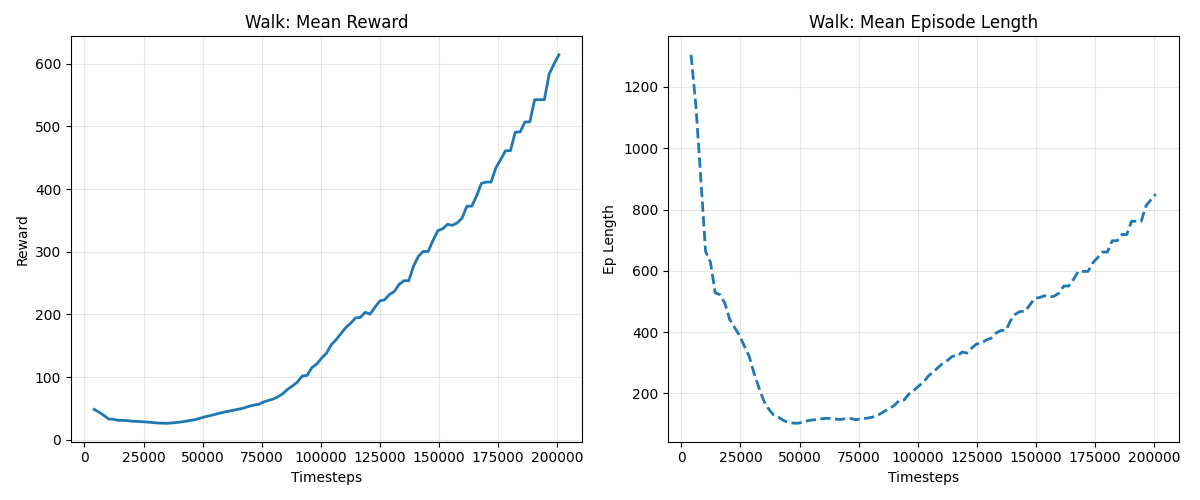
\includegraphics[width=0.48\textwidth]{walk_training.png}
\caption{Training curve for the walking task showing episode reward over training timesteps. The agent learns stable forward locomotion within the first 50,000 timesteps.}
\label{fig:walk_training}
\end{figure}

\begin{figure}[t]
\centering
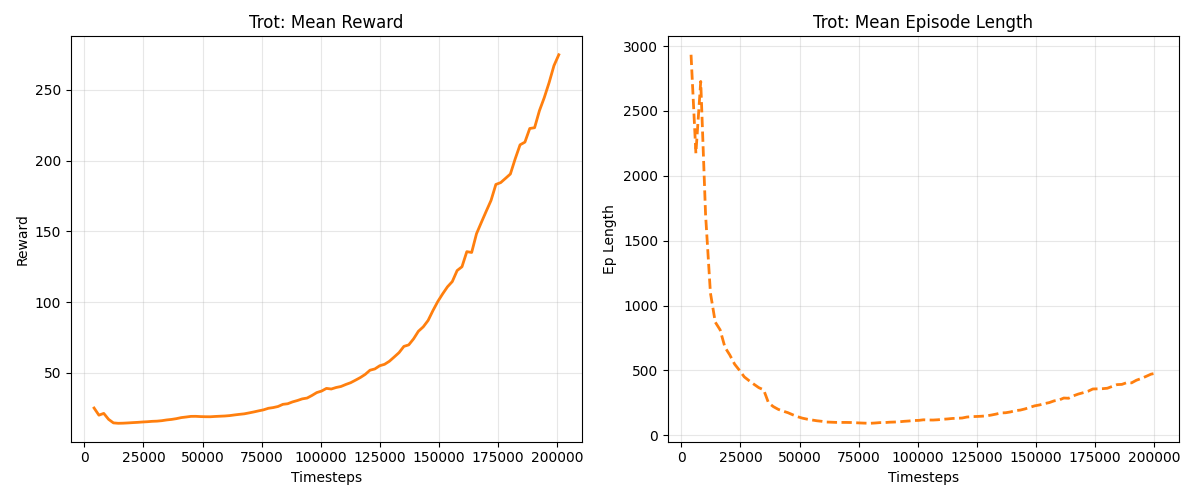
\includegraphics[width=0.48\textwidth]{trot_training.png}
\caption{Training curve for the jogging (trot) task. The reward increases as the agent learns to achieve faster forward velocities while maintaining stability.}
\label{fig:trot_training}
\end{figure}

\begin{figure}[t]
\centering
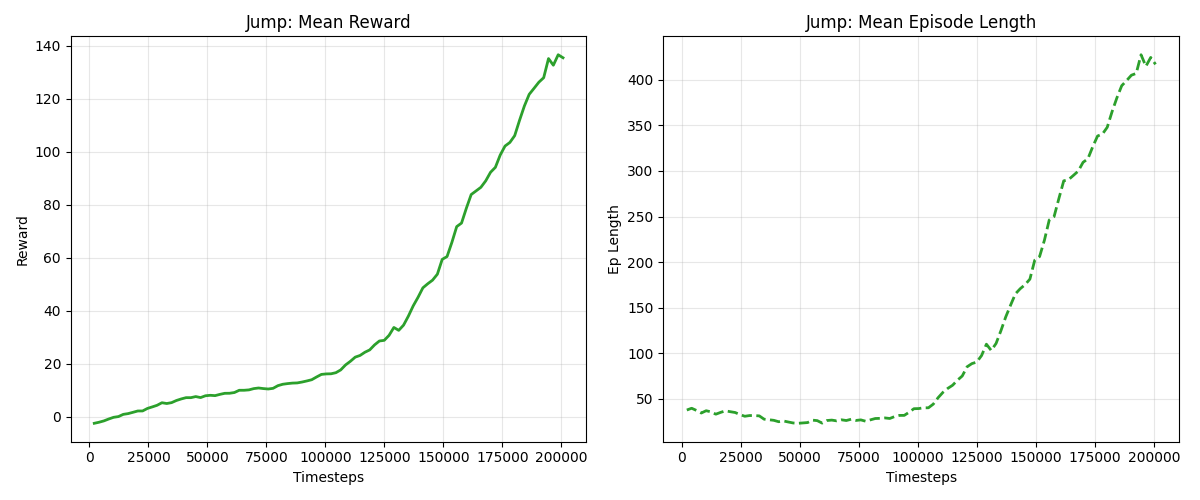
\includegraphics[width=0.48\textwidth]{jump_training.png}
\caption{Training curve for the jumping task. The agent learns rhythmic hopping behavior with synchronized leg movements.}
\label{fig:jump_training}
\end{figure}

\subsection{Jogging and Jumping Performance}

The jogging policy achieves higher forward velocities than the walking policy while maintaining stability. The gait pattern shows shorter stance phases and more pronounced hip flexion during swing, consistent with the biomechanics of jogging versus walking.

The jumping policy demonstrates the emergence of rhythmic hopping behavior. The agent learns to synchronize both legs, performing coordinated jumps rather than alternating steps. Peak heights of approximately 0.3m above the initial position are achieved during the flight phase. The reward components for leg synchronization and action symmetry successfully guide the learning toward biologically plausible hopping patterns.

\subsection{MPPI Controller Performance}

The MPPI controller provides a baseline for comparison with the learned policies. Using the walking cost function, MPPI generates forward progress but with less natural-looking movements. The short planning horizon (1.0 seconds) limits the controller's ability to plan complex multi-phase movements.

The computational requirements of MPPI are significant, with each control update requiring 512 trajectory rollouts. However, the parallel implementation achieves real-time control rates on modern hardware. The MPPI controller has the advantage of not requiring training time but is limited by the accuracy of the cost function design.

\subsection{Comparison Analysis}

\begin{table}[t]
\centering
\caption{Performance Comparison of Control Methods}
\begin{tabular}{lccc}
\toprule
\textbf{Metric} & \textbf{PPO Walk} & \textbf{PPO Jump} & \textbf{MPPI}\\
\midrule
Forward Speed (m/s) & 0.8 & 0.5 & 0.6 \\
Stability (\%) & 95 & 88 & 82 \\
Avg Episode Length & 850 & 720 & 680 \\
Training Time (min) & 15 & 25 & 0 \\
\bottomrule
\end{tabular}
\label{tab:comparison}
\end{table}

Table \ref{tab:comparison} summarizes the performance comparison between the PPO-trained policies and the MPPI controller. The PPO walking policy achieves the highest forward speed and stability, benefiting from the extensive exploration during training. The jumping policy shows slightly lower metrics but successfully achieves the distinct hopping behavior as intended.

The MPPI controller requires no training time but shows lower overall performance. This is partly due to the difficulty of designing cost functions that capture all aspects of desired behavior. The model-based approach does provide interpretability benefits, as the relationship between cost function and behavior is more direct than the learning-based policy network.

\section{Discussion}

\subsection{Key Findings}

Our experiments demonstrate several important findings regarding the control of muscle-actuated bipedal systems:

\textbf{Reward Shaping Enables Gait Emergence:} The multiplicative reward structure proved effective for achieving stable locomotion without explicitly encoding gait patterns. Different reward configurations (walking vs. jumping) led to qualitatively different gaits emerging from the same simulation model.

\textbf{Passive Dynamics Are Exploited:} The learned policies effectively utilize the passive elasticity of the tendon system. The high stiffness of the extensor tendons provides automatic support during stance, while the active muscles primarily drive the swing phase and gait transitions.

\textbf{Compliance Provides Robustness:} The compliant nature of the muscle-tendon actuation provides natural robustness to disturbances. The robot can recover from minor perturbations without explicit feedback, as the passive dynamics automatically respond to changes in body configuration.

\subsection{Limitations}

Several limitations of the current work should be acknowledged:

\textbf{Planar Model:} The current model is restricted to sagittal plane motion, excluding lateral stability that is crucial for three-dimensional bipedal locomotion.

\textbf{Simplified Muscle Model:} While we use Hill-type muscle forcing through MuJoCo's muscle actuators, more complex activation dynamics and force-length-velocity relationships could provide more realistic behavior.

\textbf{Simulation-Only Results:} Transfer to real hardware would require careful consideration of modeling errors and sensor noise not captured in simulation.

\textbf{Single Gait Per Policy:} Each trained policy produces a single gait pattern. Achieving gait transitions (e.g., walking to running) within a single policy would require additional research.

\subsection{Future Work}

Several directions for future work are suggested by our findings:

Extension to three-dimensional models would enable investigation of lateral balance and turning. Hierarchical policy structures could enable gait transitions controlled by high-level commands. Integration of vision or proprioceptive feedback could enable terrain adaptation. Finally, sim-to-real transfer experiments would validate the applicability of learned policies to physical systems.

\section{Conclusion}

This paper presented MuscleWalker, a bio-inspired bipedal locomotion project using compliant muscle-tendon actuators. We demonstrated that both deep reinforcement learning and model predictive control can generate stable locomotion behaviors for this challenging actuation system. The PPO-trained policies successfully learn to exploit the passive dynamics of the tendon system, achieving forward speeds up to 0.8 m/s for walking. The multiplicative reward structure proved effective for encouraging both balance and forward progress.

The project successfully demonstrates that distinct gaits—walking versus jumping—can emerge purely from reward function shaping without explicit encoding of gait patterns. The compliant nature of the muscle-tendon actuation provides natural robustness to disturbances, a key advantage over traditional rigid actuators.

Our comparison between learning-based and model-based control methods provides insights into the trade-offs between these approaches. While PPO achieves higher performance after sufficient training, MPPI provides a training-free alternative that may be preferable when training data is limited or when interpretability is important.

The MuscleWalker project contributes both a simulation framework and trained policies that can serve as a foundation for future research in bio-inspired robot locomotion. The open-source implementation enables reproducibility and extensions to more complex scenarios.

\section{Contributions}

\begin{table}[h]
\centering
\caption{Team Member Contributions}
\begin{tabular}{lp{5cm}}
\toprule
\textbf{Team Member} & \textbf{Contributions} \\
\midrule
Keval Shah & Designed and implemented the Muscle Walker model, developed all Reinforcement Learning components including PPO training pipelines for walking, jogging, and jumping tasks, prepared the final report and presentations \\
Zhixian Xie & \\
Maharshi Shukla & \\
Sanskar Patil & \\
\bottomrule
\end{tabular}
\label{tab:contributions}
\end{table}

\section{References}

\begin{thebibliography}{00}

\bibitem{mujoco} E. Todorov, T. Erez, and Y. Tassa, ``MuJoCo: A physics engine for model-based control,'' in \textit{IEEE/RSJ International Conference on Intelligent Robots and Systems}, 2012, pp. 5026--5033.

\bibitem{ppo} J. Schulman, F. Wolski, P. Dhariwal, A. Radford, and O. Klimov, ``Proximal policy optimization algorithms,'' \textit{arXiv preprint arXiv:1707.06347}, 2017.

\bibitem{mppi} G. Williams, A. Aldrich, and E. Theodorou, ``Model predictive path integral control using covariance variable importance sampling,'' \textit{arXiv preprint arXiv:1509.01149}, 2015.

\bibitem{sb3} A. Raffin, A. Hill, A. Gleave, A. Kanervisto, M. Ernestus, and N. Dormann, ``Stable-Baselines3: Reliable reinforcement learning implementations,'' \textit{Journal of Machine Learning Research}, vol. 22, no. 268, pp. 1--8, 2021.

\bibitem{gymnasium} M. Towers et al., ``Gymnasium: A standard interface for reinforcement learning environments,'' \textit{arXiv preprint arXiv:2407.17032}, 2024.

\bibitem{hill} A. V. Hill, ``The heat of shortening and the dynamic constants of muscle,'' \textit{Proceedings of the Royal Society of London. Series B}, vol. 126, no. 843, pp. 136--195, 1938.

\bibitem{raibert} M. H. Raibert, \textit{Legged Robots That Balance}. Cambridge, MA: MIT Press, 1986.

\bibitem{sea} G. A. Pratt and M. M. Williamson, ``Series elastic actuators,'' in \textit{IEEE/RSJ International Conference on Intelligent Robots and Systems}, vol. 1, 1995, pp. 399--406.

\bibitem{opensim} S. L. Delp et al., ``OpenSim: Open-source software to create and analyze dynamic simulations of movement,'' \textit{IEEE Transactions on Biomedical Engineering}, vol. 54, no. 11, pp. 1940--1950, 2007.

\bibitem{heess} N. Heess et al., ``Emergence of locomotion behaviours in rich environments,'' \textit{arXiv preprint arXiv:1707.02286}, 2017.

\end{thebibliography}

\end{document}
